\begin{TP}[Triominos avec les angles]


\textbf{1\up{ère} étape : calculer et justifier}

\begin{enumerate}
\item Voici six figures. Pour chacune d'elles, calculez, en justifiant votre calcul, l'angle marqué par un point d'interrogation. (Les droites d'une même couleur sont parallèles.)

\begin{center}
    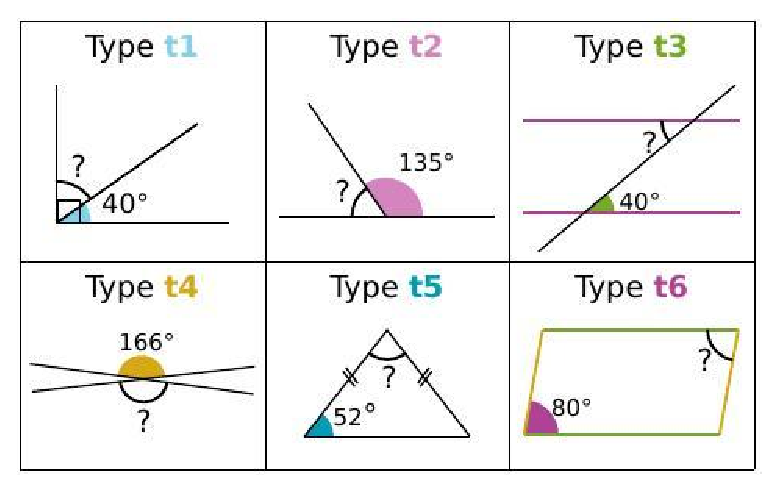
\includegraphics[width=.6\linewidth]{tabImage}
\end{center}


\item Voici six énoncés. Pour chacun d'eux, répondez à la question en justifiant la réponse :

\begin{center}
    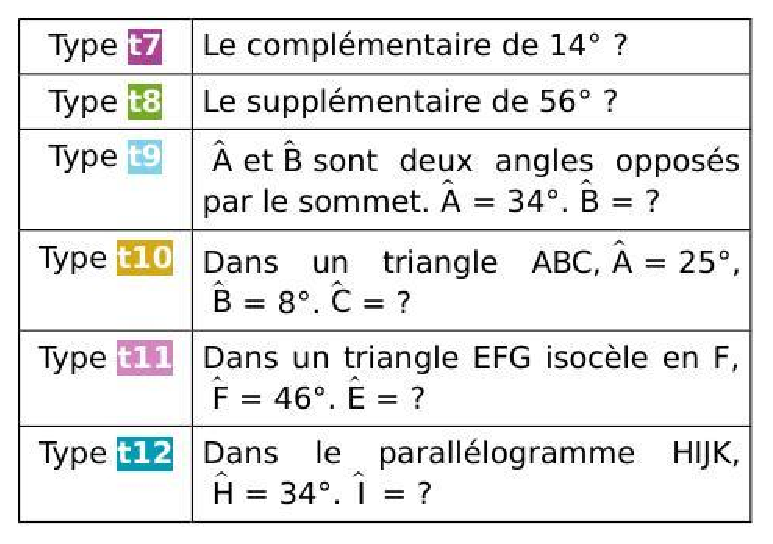
\includegraphics[width=.6\linewidth]{tabType}
\end{center}


\vspace{1em}\textbf{2\up{e} étape : construction des triominos}\vspace{1em}

\item \label{AtpTabType} Voici un tableau qui va vous permettre de construire le jeu de triominos. 

\begin{center}
    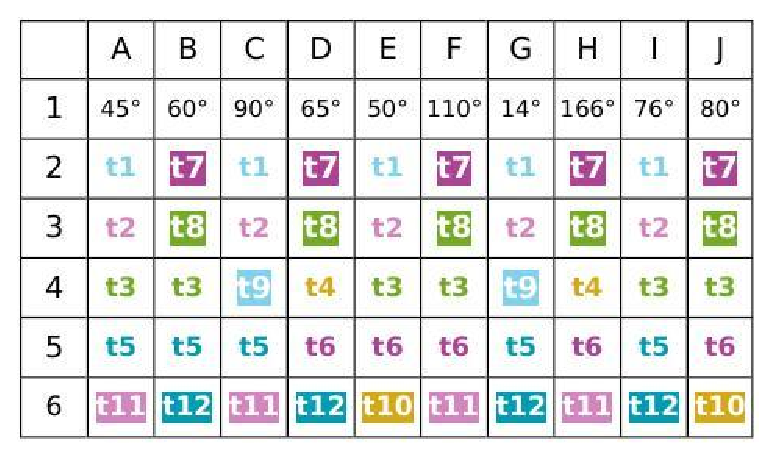
\includegraphics[width=.6\linewidth]{tableau}
\end{center}

Toutes les cases d'une même colonne renvoient à l'angle indiqué en ligne 1. Par exemple, les cases F2, F3... renvoient à un angle de 110°.

Pour le type \textbf{t3}, mettez aussi des exemples d'angles correspondants.

\item Dans une feuille blanche au format A4, construisez 10 triangles équilatéraux de 9 cm de côté. Utilisez une seconde feuille pour obtenir 20 triominos au total. Complétez chacun d'eux avec les énoncés ou constructions indiqués dans le tableau de la question \ref{AtpTabType}. en respectant l'ordre donné ci-dessous. Pour vous aider, voici un exemple pour le premier triomino de la série :

\hfill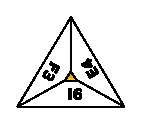
\includegraphics[width=.15\linewidth]{tp7} \hfill 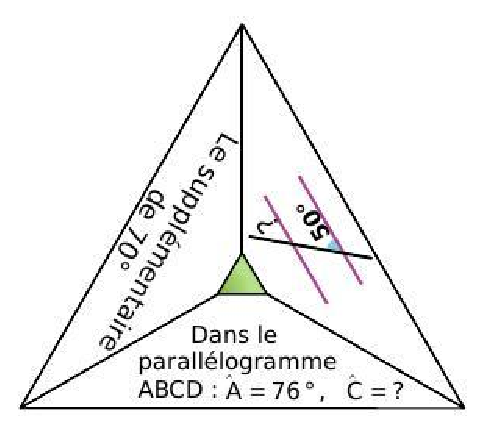
\includegraphics[width=.3\linewidth]{tp8}\hfill\phantom{.}
 
\begin{center}
    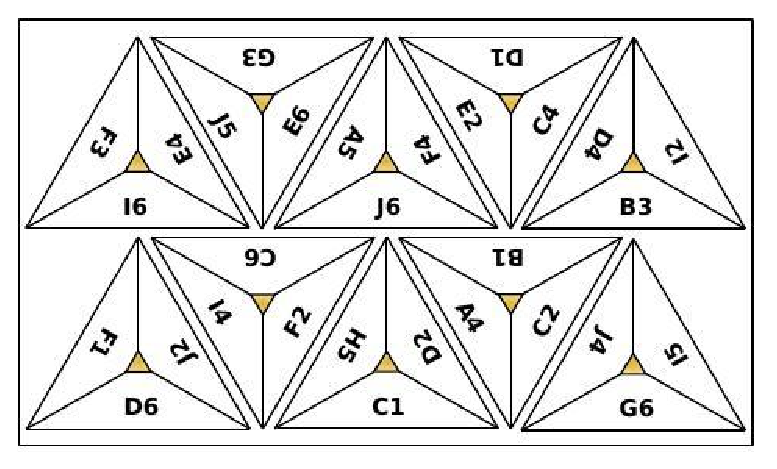
\includegraphics[width=.75\linewidth]{tp9}
    
    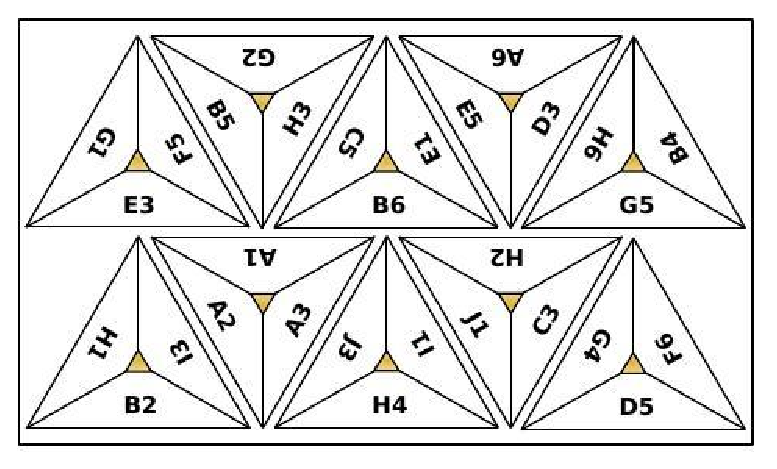
\includegraphics[width=.75\linewidth]{tp10}
\end{center}

\vspace{1em}\textbf{3\up{e} étape : par équipe de deux joueurs}\vspace{1em}

Retournez tous les triominos pour former la pioche. Chaque joueur en prend quatre.      

Un triomino est tiré dans la pioche pour servir de départ. Chaque joueur place à son tour un triomino. (Les côtés qui se touchent doivent correspondre à des angles égaux.)

Si le joueur ne peut pas jouer, il passe son tour \textbf{et} pioche. Le premier joueur qui n'a plus de triomino est déclaré vainqueur.

\textbf{Attention} : si un joueur se trompe en plaçant un triomino, il doit le reprendre et tirer un triomino supplémentaire dans la pioche ; c'est alors à son adversaire de jouer...
\end{enumerate}

\end{TP}